\section{Memory Networks}
%TODO: General introduction about the need for explicit memory.
Memory Networks (MemNet) are a class of models
that combine inference with long-term memory. Unlike Recurrent Neural Networks
(RNN) that model language \citep{mikolov2010recurrent}, and their variants with
Long Short-Term Memory (LSTM) \citep{hochreiter1997long}, MemNets have an explicit
memory component with read and write functions. While the original MemNet model 
proposed by \cite{weston2014memory}, MemNN required explicit supervision
for selecting the relevant parts of the memory, \citep{sukhbaatar2015end}
proposed a end-to-end variant (MemN2N) where the memory selection component is
trained jointly with the rest of the network. These were previously used for
answering questions that require reasoning over multiple context sentences,
both in simulated \citep{bordes2010towards} and large-scale
\citep{fader2013paraphrase} scenarios.

In this chapter, we use the term \textit{memory network},
or the abbreviation \textit{MemNet}, to refer to any neural network model with an explicit memory component
that can be read from or written to. Our focus is mostly on the general class of models. Wherever necessary,
we refer to the original memory network model
proposed by \cite{weston2014memory} as \textit{MemNN} and the end to end model by \cite{sukhbaatar2015end}
as MemN2N.


\begin{figure*}
\begin{center}
  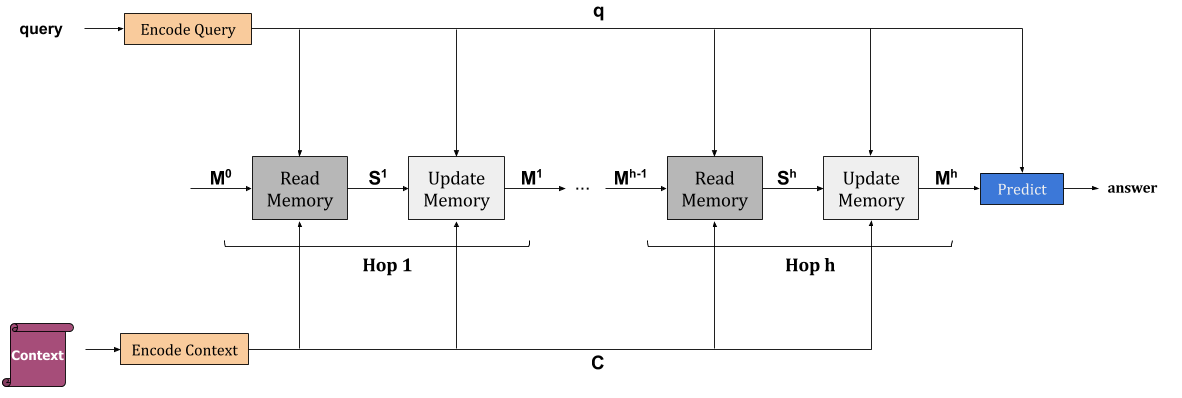
\includegraphics[width=6.5in]{figures/memory_network_generic.png}
  \caption{Schematic showing a generic view of end-to-end memory network}
  \label{fig:memnet}
  \end{center}
\end{figure*}
Figure~\ref{fig:memnet} shows the setup of a generic MemNet. It takes as
input a set of $N$ context sentences indexed as $\{c_i\}_{i=1}^N$, such that
$c_i$ is a vector containing the indices of words in the $i^\text{th}$ sentence.
The sentences are then encoded using the \texttt{EncodeContext} function to
produce the matrix $C \in \mathbb{R}^{n \times d}$, where each row $C[i]$ is the
encoding of sentence $c_i$. In addition, the model also takes as input a query
indexed as $q$, which is a vector containing the indices of the words in the
query similar to $c_i$ vectors. The query is encoded using \texttt{EncodeQuery}
to produce $u^0 \in \mathbb{R}^d$. The memory network can have multiple memory
layers, corresponding to multiple hops. At each hop, a memory layer receives as
input the output from the previous hop $u^{h-1}$, which is passed to the
\texttt{SelectMemory} function, which uses an attention mechanism to select the
relevant parts of the encoded context, conditioned on $u^{h-1}$ and produces
a summary $s^h$, of the context encoding for the current hop. $s^h$ is then
passed to \texttt{UpdateMemory} along with $u^{h-1}$, to produce the updated
memory representation $u^h$ for the current hop. It has to be noted that the
initial $u^0$ is the encoding of the query itself. Finally, an answer is
predicted by passing the query encoding $u^0$, and the summary of the
context, $s^H$ from the final hop $H$ to the \texttt{PredictAnswer} function.

It can be seen that MemN2N fits into this setup with the following
configuration:
% TODO(pradeep): MemN2N actually has two Embedding matrices encoding background
% for input and output. Also, there is another variant which encodes positions of
% the words too.
\begin{flalign*}
&\texttt{EncodeQuery}(q) = \text{Embedding}_q(q) \\
&\texttt{EncodeContext}(c_i) = \text{Embedding}_c(c_i) \\
&\texttt{SelectMemory}(u^{h-1}, C) = \text{softmax}(C.u^{h-1}).C \\
&\texttt{UpdateMemory}(u^{h-1}, s^h) = u^{h-1} + s^h \\
&\texttt{PredictAnswer}(u_0, s^H) = \text{softmax}(W.s^H)
\end{flalign*}
where $\text{Embedding}_q(.)$ and $\text{Embedding}_c(.)$ are simply bag of
words models that aggregate the vector representations of all the words given by
the indices in the input. $W \in \mathbb{R}^{V \times d}$ is a parameter of the
answer prediction function, causing the softmax to be over the vocabulary size
$V$. Note that in MemN2N, $u^0$ is not an argument of \texttt{PredictAnswer}.

In this chapter, we focus on problems where the context is not well-defined, and needs to
be retrieved for a big corpus. Accordingly, we propose to add an additional
\texttt{RetrieveContext} module to our generic MemNet architecture.
Particularly, we are interested in developing MemNet models that
can figure out whether the available context is sufficient to make a prediction. We first
describe a target dataset for our model, and then list the issues we propose to address.

\section{Science Question Answering}
The ScienceQA dataset we use here is significantly different from the
QA datasets previously used to test memory networks, and requires more complex
reasoning. One example of such question is shown below.
%TODO(pradeep): Make this a table?
\begin{itemize}
\item Astronauts weigh more on Earth than they do on the moon because
\begin{enumerate}[(a)]
 \item they have less mass on the moon
 \item their density decreases on the moon
 \item the moon has less gravity than Earth
 \item the moon has less friction than Earth
\end{enumerate}
\end{itemize}
%TODO(pradeep): Say more things about the nature of the problem.
The text relevant to questions like this may contain a single sentence that
has the information to answer this question, like this:
\begin{itemize}
 \item People weigh more on some planets than others because of differences in gravity.
\end{itemize}

Or it may span multiple sentences like this:
\begin{itemize}
 \item Moon's gravity is less than that of Earth.
 \item Weight of a person depends on the gravity of the planet.
\end{itemize}

Or in other cases, the text may not contain the relevant answer at all. Hence, this setup
requires an module in addition to the ones mentioned that retrieves relevant content from
the corpus. However, as the size of the context increases, it becomes more and more expensive to reason over
it. Also, increased context size may add noise to prediction process. Hence, it is important to
retrieve context conservatively, and the model should reason whether the retrieved context
is sufficient to produce an answer.

\paragraph{Question Answering as Textual Entailment} In our proposed setup, we
cast the problem of deciding whether the given context is sufficient to answer the question, as a
textual entailment problem. That is, given a multiple choice question with answer options, we
convert the combination of the question and each of the options into a
statement, and check whether the statement can be entailed from relevant
background information. Given this setup, the \texttt{PredictAnswer} function
essentially becomes an entailment function. If none of the question-option combinations
can be entailed from (or contradicted by) the retrieved context, we retrieve more context.

\subsection{Proposed Algorithm}
Based on the ideas described so far, we now present the proposed algorithm, \textsc{AdaptiveRead}
to read and reason, while choosing to retrieve or predict depending on the sufficiency
of the context available.

\begin{algorithm}[H]
 \KwIn{$L$: large corpus, $q$: question}
 \KwOut{$a$: answer}
 $ContextSize = k$ \;
 $C = \texttt{RetrieveContext}(q, L, ContextSize)$, the top $k$ relevant sentences from the corpus\;
 \While{$ContextSize < MaxContextSize$} {
  \eIf{$\texttt{EntailsOrContradicts}(C, q)$}{
    $a = \texttt{PredictAnswer}(C, q)$ \;
    return $a$
  }{
    $ContextSize += k$ \;
    $C = \texttt{RetrieveContext}(q, L, ContextSize)$ \;
  }
 }
 \caption{\textsc{AdaptiveRead} algorithm that learns when to stop retrieving context}
\end{algorithm}

This algorithm shares some similarities with the \textit{ReasoNet} model
proposed by \cite{shen2016reasonet}, but the main difference is that while ReasoNet learns to
stop performing additional hops, the proposed algorithm learns to stop retrieving additional context.

\subsection{Potential Issues}
We identify the following potential issues in building \textsc{AdaptiveRead}.
\begin{enumerate}
 \item \textbf{Scalability to large corpora}: Depending on the complexity of \texttt{PredictAnswer}, reasoning
 over large corpora may prove to be intractable. Earlier work in solving this problem involves building
 hierarchical models \cite{chandar2016hierarchical,choi2016hierarchical}. While \cite{chandar2016hierarchical}
 build a hierarchical memory network that uses a simple dot product for \texttt{RetrieveContext} and \texttt{SelectMemory},
 and thus use maximum inner product search (MIPS) to do them efficiently, \cite{choi2016hierarchical} perform summarization
 to retrieve context followed by answer prediction. We can use some of their ideas to make \texttt{RetrieveContext} a simpler
 process, and \texttt{SelectMemory} a more expensive one.
 
 \item \textbf{Difficulty in training}: Clearly, \textsc{AdaptiveRead} makes a hard choice between retrieving context and
 predicting an answer, thus making it impossible to train the model end-to-end using back-propagation. \cite{shen2016reasonet}
 and \cite{choi2016hierarchical} get around this problem using REINFORCE \cite{williams1992simple} algorithm.
\end{enumerate}


% \subsection{Preliminary Results}
% We performed some preliminary experiments to understand the 
% We now show some preliminary results of our memory network implementation on science question answering using MemN2N architecture with following change in configuration:
% \begin{flalign*}
% &\texttt{PredictAnswer}(u_0, s^H) = \texttt{HeuristicMatch}(u_0, s_h)
% \end{flalign*}
% where \texttt{HeuristicMatch}(.) is the heuristic matching function proposed by \cite{mou2015recognizing} for textual entailment, also used for our experiments with SNLI data in 
% Chapter~\ref{chapter:ontolstm}. The dataset used for these experiments is questions collected from 4th and 8th grade science text books.
% Context for each question was obtained as follows. We built a Lucene index over a big collection of sentences related to general science from various sources and extracted relevant background sentences for each question by querying it. For each of the
% options, we query the Lucene index with a combination of the option text and the question. We thus transform questions like the one shown above into four entailment problems where the combination of the
% question and one of the options is the hypothesis and the relevant background sentences are the premises. The final answer is picked by selecting the option (combined with the question) that has the highest
% entailment score. This is done by passing the final entailment scores through a softmax layer.
% 
% Preliminary results using our model are shown in Table~\ref{tab:memnet_qa_results}, using two different encoders
% to encode the input sentences and background. We also show the accuracy of a baseline system based on Lucene, that selects for every question, the option that results in the highest relevance score in the process
% described above for retrieving background sentences. It can be seen that the simple baseline does better than the memory network model.
% 
% \begin{table}
%     \centering
%     \begin{tabular}{|l|c|}
%     \hline
%     \textbf{Encoder} & \textbf{Test Acc.}\\
%     \hline
%     BOW & \% \\
%     GRU & 38.8\% \\
%     \hline
%     \hline
%     \textbf{Lucene baseline} & 41.1\% \\
%     \hline
%     \end{tabular}
%     \caption{Results of our Memory Network on ScienceQA in comparison with a Lucene baseline}
%     \label{tab:memnet_qa_results}
% \end{table}
% 
% \subsection{Analysis}
% 
% \subsection{Proposed Work}


